%\documentclass[a4j,twocolumn,uplatex]{jsarticle}
\documentclass[a4j,twocolumn,uplatex]{jarticle}

\usepackage[dvipdfmx]{graphicx}
\usepackage{wrapfig}	
\usepackage[dvipdfmx]{graphicx}
\usepackage{url}
\usepackage{here}
\usepackage{subfigure}
\setlength{\textheight}{275mm}
\headheight 5mm
\topmargin -30mm
\textwidth 185mm
\oddsidemargin -15mm
\evensidemargin -15mm
\pagestyle{empty}
\def\Vec#1{\mbox{\boldmath $#1$}}
\usepackage[dvipdfmx]{graphics}
\usepackage{comment}

\usepackage{subfigure}



\begin{document}
\title{Processingによるホイヘンスの原理の視覚化}
\author{情報科学科 西谷研究室3518 村上 大貴}
\date{}
\maketitle
\section{はじめに}
現在,政府は2020年を目標に中学および高等学校の全生徒がタブレットを携行するという計画を立てている\cite{tablet}.
タブレット端末を学習に活用することが出来れば,
従来指導が難しいとされていた教科も分かり易く指導を行える可能性が生まれる.
そのような状況でタブレット端末の特性を活かした学習コンテンツの作成が喫緊の課題であると考える.

タブレット端末の利点としてインタラクティブな教材を使用できる点が挙げられるが,
このような教材が効力を発揮する教科の一つに物理がある.
物理現象は,文章や数式による記述では非常に理解しづらいものが存在する.
例えば,波の進み方の原理を説明するホイヘンスの原理は,
実世界には存在しない素元波という概念を用いて波面を決定していく.
しかし,実世界にないが故に直観的な理解を得るのは難しい.
これを直観的に理解させ,学習を促進する手段として,物理現象の視覚化が適していると考える.
本研究では,素元波の発生と,波面の決定をプログラムにより視覚化することを目標とする.プログラムはProcessing言語により記述する.
%これによりホイヘンスの原理を理解することを容易にした上,
%この原理により説明できる,波の反射,屈折,回折を深く理解できることを意図している.
\vspace{-4mm}

\section{Processingについて}
Processing(プロセッシング)とはオープンソースのプログラミング言語およびソフトウェア開発環境である.
Processing言語は以下に挙げるような特徴を有している\cite{ishikawa}.
\begin{enumerate}
\item 基本文法はJavaをベースに記法を簡単化したものであり,
インタラクティブソフトウェアやビジュアルプレゼンテーションを容易に実現することに特化している.
\item 環境構築が非常に容易かつ無償で行える.
\item Windows, iOS, Androidのタブレット端末で用いられる3つのプラットフォーム全てで動作する. %//なんで動作するかを調べる
\end{enumerate}
これらの理由から,本研究で使用するプログラミング言語に最も適していると考える.
\vspace{-4mm}
\section{ホイヘンスの原理}
教科書では「1つの波面上の全ての点は,それらを波源とする球面波(素元波)を発生させ,素元波の共通に接する面が次の瞬間の波面となる.これをホイヘンスの原理という」と述べている.\cite{kyoukasyo}.
波の持つ屈折,回折,反射の性質は,この原理により説明できる.
屈折は,媒質ごとに発生する素元波の波長が異なる事から説明できる.
回折は波が隙間(スリット)を通る際,
隙間の幅が広い時と狭い時で,素元波の進行方向が変わることから,
回折の度合いが違うことを説明できる.
反射は,波がはね返る点から生じる素元波の共通接線を新波面とすることにより説明できる.
\vspace{-6mm}

\begin{figure}[htbp]
\subfigure[波の屈折]{\mbox{\raisebox{1mm}{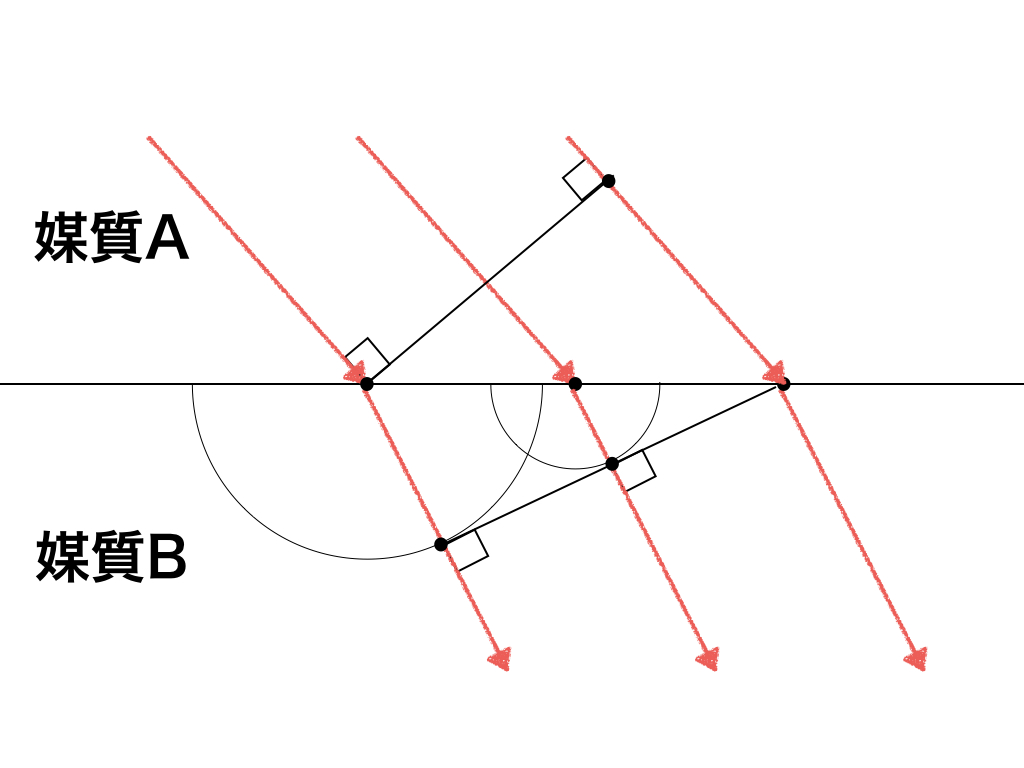
\includegraphics[keepaspectratio, scale = 0.11]{./refraction.png}}}}
\subfigure[波の回折]{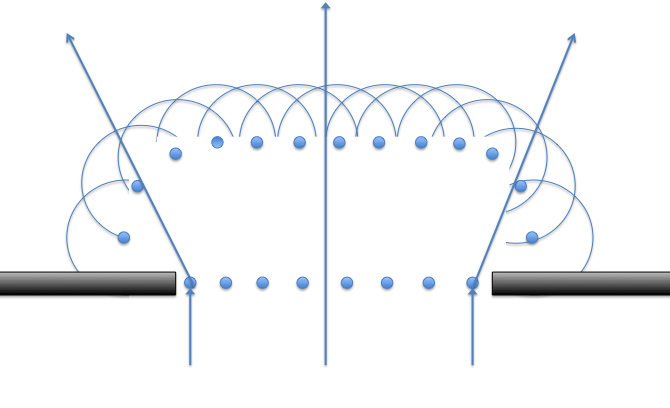
\includegraphics[keepaspectratio, scale = 0.18]{./diffraction.png}}
\subfigure[波の反射]{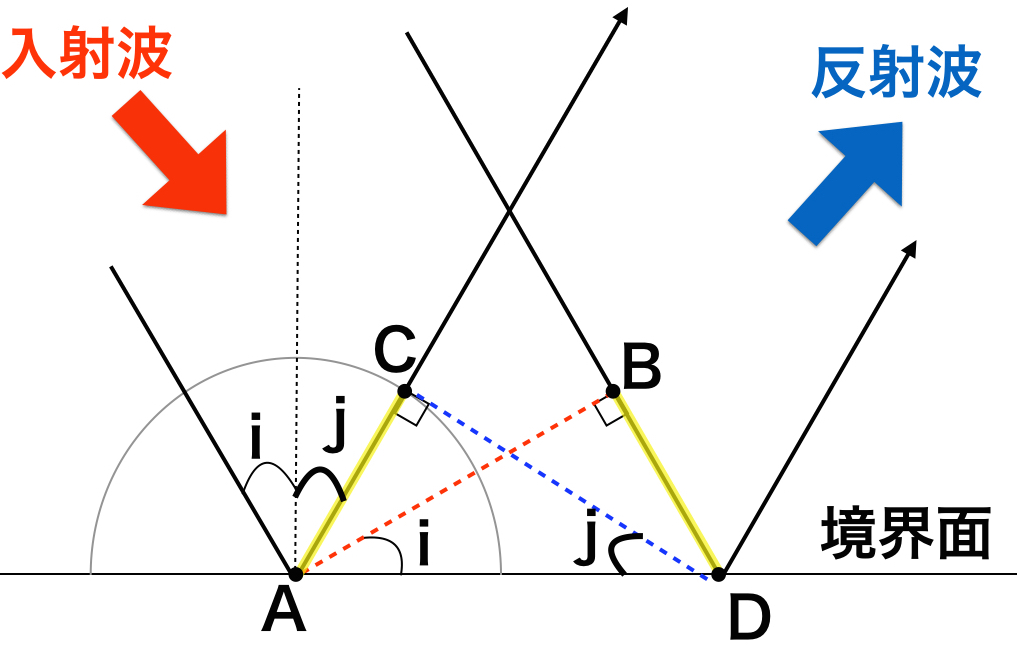
\includegraphics[keepaspectratio, scale = 0.14]{./reflection.png}}
\caption{{\footnotesize 波の性質と素元波 }}
\label{fig:thomson2clausius}
\end{figure}
\vspace{-7mm}

\section{今後の課題}
%中村らのホイヘンスの原理の説明は,
%素元波の共通に接する面が次の瞬間の波面であるとしている.
%これは素元波上に無限に素元波を発生させる点があるという前提で述べていると言える.
%もし素元波を発生させる点が有限であれば,
%発生する素元波の一つ一つを囲う線が次の瞬間の波面である.
%これを視覚化するプログラムを作成する.
現在,ホイヘンスの原理を視覚化するプログラムは完成していないので,これを完成させる.
そしてこののプログラムを元として,波の屈折,回折,反射の視覚化を試みる.
また物理の苦手な生徒,物理に関心を持っていないような生徒でも原理を的確に理解できるように以下のような機能を実装する.
\begin{enumerate}
\item 素元波の点源数を自由に変更可能とする.
\item 素元波の表示切り替えを可能とする
\item 波の強度の表示を描画線の太さや色などで表現する.
\end{enumerate}

\vspace{-5mm}
\begin{thebibliography}{9}
\bibitem{tablet}「教育の情報化ビジョン 〜21世紀にふさわしい学びと学校の創造を目指して〜」文部科学省,p34 \url{http://www.mext.go.jp/b_menu/houdou/23/04/__icsFiles/afieldfile/2011/04/28/1305484_01_1.pdf}.
\bibitem{ishikawa} 石川将人,北卓人,大須賀公一. Arduino/Processingを用いたシステム制御実験のラピッドプロトタイピング. 自動制御連合講演会講演論文集 53(0), 2010. p.247 
\bibitem{kyoukasyo} 中村 英二ほか ,「物理I」, 学習社 2004).


\end{thebibliography}
\end{document}

